\documentclass[12pt]{article}
\usepackage{gensymb}
\usepackage{float}
\usepackage{amsmath}
\usepackage{graphics}
\usepackage{graphicx}
\graphicspath{{storage/self/primary/Download/asgnt2/fig}}
\providecommand{\brak}[1]{\ensuremath{\left(#1\right)}}
\providecommand{\myvec}[1]{\ensuremath{\begin{pmatrix}#1\end{pmatrix}}}
\newcommand\norm[1]{\left\Vert#1\right\Vert}
\let\vec\mathbf
\begin{document}
\title{\textbf{ASSIGNMENT-12.11.2.3}}
\date{}
\maketitle
\textbf{Question :} Show that the line through the points \brak{4,7,8},\brak{2,3,4} is parallel to the line through the points\brak{-1,-2,1},\brak{1,2,5}.

\textbf{Solution :}
For line passing through \brak{4,7,8},\brak{2,3,4},the direction vector,\begin{align}
    \vec{m_1}&=\myvec{-2\\-4\\-4}
\end{align}
For line passing through \brak{-1,-2,1},\brak{1,2,5},the direction vector,\begin{align}
    \vec{m_2}&=\myvec{2\\4\\4}
\end{align}
Therefore,the lines are parallel to each other.
\begin{figure}[H]
    \centering
    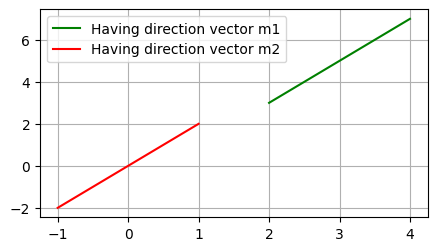
\includegraphics[width=\columnwidth]{fig/12.11.2.3.png}
    \caption{}
    \label{12.11.2.3}
\end{figure}
\end{document}
